\documentclass[14pt, a4paper]{extarticle}
\usepackage{GOST}
\usepackage{array}
\usepackage{verbatim}
\usepackage[detect-all]{siunitx}
\usepackage{amsmath}
\usepackage{amssymb}
\usepackage[utf8]{inputenc}
\usepackage{hyperref}
\usepackage{tempora}

\makeatletter
\renewcommand\@biblabel[1]{#1.}
\makeatother

\usepackage{listings}
\lstset{ 
	language=python,
	basicstyle=\small\sffamily, 
	numbers=left, 
	numberstyle=\tiny,
	stepnumber=1,
	numbersep=5pt,
	showspaces=false,            
	showstringspaces=false,      
	showtabs=false,             
	frame=single,            % рисовать рамку вокруг кода
	tabsize=4,      
	commentstyle=\color{green},
	keywordstyle=\color{blue}\textbf,
	numberstyle=\scriptsize\color{gray}, % the style that is used for the line-numbers
	rulecolor=\color{black},
	captionpos=t,
	breaklines=true,         % автоматически переносить строки 
	breakatwhitespace=false, % переносить строки по пробелу
	escapeinside={\#*}{*)} 
}


\usepackage{pgfplots}
\usepackage{filecontents}
\usetikzlibrary{datavisualization}
\usetikzlibrary{datavisualization.formats.functions}

\begin{document}
	
\begin{table}[ht]
	\centering
	\begin{tabular}{|c|p{400pt}|} 
		\hline
		\begin{tabular}[c]{@{}c@{}} 
\includegraphics[scale=1]{source/b_logo.jpg} \\\end{tabular} &
		\footnotesize\begin{tabular}[c]{@{}c@{}}\textbf{Министерство~науки~и~высшего~образования~Российской~Федерации}\\\textbf{Федеральное~государственное~бюджетное~образовательное~учреждение}\\\textbf{~высшего~образования}\\\textbf{«Московский~государственный~технический~университет}\\\textbf{имени~Н.Э.~Баумана}\\\textbf{(национальный~исследовательский~университет)»}\\\textbf{(МГТУ~им.~Н.Э.~Баумана)}\\\end{tabular}  \\
		\hline
	\end{tabular}
\end{table}
\noindent\rule{\textwidth}{4pt}
\noindent\rule[14pt]{\textwidth}{1pt}
\hfill 
\noindent
\makebox{ФАКУЛЬТЕТ~}%
\makebox[\textwidth][l]{\underline{~«Информатика и системы управления»~~~~~~~~~~~~~~~~~~~~~~~~~~~~~~~~~}}%
\\
\noindent
\makebox{КАФЕДРА~}%
\makebox[\textwidth][l]{\underline{~«Программное обеспечение ЭВМ и информационные технологии»~}}%
\\

\begin{center}
	\vspace{1.5cm}
	{\bf\huge Отчёт\par}
	{\bf\Large по лабораторной работе № 7\par}
	\vspace{0.7cm}
\end{center}


\noindent
\makebox{\large{\bf Название:}~~~}
\makebox[\textwidth][l]{\large\underline{~Поиск по словарю~}}\\

\noindent
\makebox{\large{\bf Дисциплина:}~~~}
\makebox[\textwidth][l]{\large\underline{~Анализ алгоритмов~~~~~~~~~~~~~~~~~~~~~~~~~~}}\\

\vspace{1.5cm}
\noindent
\begin{tabular}{l c c c c c}
	Студент      & ~ИУ7-55Б~               & \hspace{2.5cm} & \hspace{2cm}                 & &  Д.О. Склифасовский \\\cline{2-2}\cline{4-4} \cline{6-6} 
	\hspace{3cm} & {\footnotesize(Группа)} &                & {\footnotesize(Подпись, дата)} & & {\footnotesize(И.О. Фамилия)}
\end{tabular}

\noindent
\begin{tabular}{l c c c c}
	Преподователь & \hspace{5cm}   & \hspace{2cm}                 & & ~~~~~~Л.Л. Волкова~~~~~~\\\cline{3-3} \cline{5-5} 
	\hspace{3cm}  &                & {\footnotesize(Подпись, дата)} & & {\footnotesize(И.О. Фамилия)}
\end{tabular}

\vspace{0.6cm}
\begin{center}	
	\vfill
	\large \textit {Москва, 2020}
\end{center}

\thispagestyle {empty}
\pagebreak

% СОДЕРЖАНИЕ 
\clearpage
\tableofcontents

% ВВЕДЕНИЕ
\clearpage
\section*{Введение}
\addcontentsline{toc}{section}{Введение}
Цель работы: изучение алгоритмов поиска слов в словаре\par
В ходе лабораторной работы требуется:
\begin{enumerate}
	\item[1)] описать алгоритм полного перебора;
	\item[2)] описать алгоритм двоичного поиска;
	\item[3)] описать алгоритм поиска слов по сегментам;
	\item[4)] реализовать 3 алгоритма поиска по словарю;
	\item[5)] провести замеры времени работы алгоритмов.
\end{enumerate}\par

% АНАЛИТИЧЕСКИЙ РАЗДЕЛ
\clearpage
\section{Аналитический раздел}
В данном разделе представлено описание трех выбранных алгоритмов.
\subsection{Общие сведения}
Словарь — книга или любой другой источник, информация в котором упорядочена c помощью разбивки на небольшие статьи, отсортированные по названию или тематике. Различают энциклопедические и лингвистические словари.
С развитием компьютерной техники всё большее распространение получают электронные словари и онлайн-словари.
Первым русским словарём принято считать Азбуковник, помещённый в списке Кормчей книги 1282 года и содержащий 174 слова. Задача состоит в поиске слов из словаря в случайных данных любого размера(напр. в файле).
Поскольку словарь меняется редко, то можно его подготовить (напр. отсортировать, создать дерево итд). Это зависит от алгоритма поиска, который будет использован. 
\subsection{Алгоритм полного перебора}
Алгоритм полного перебора — это алгоритм разрешения математических задач, который можно отнести к классу способов нахождения решения рассмотрением всех возможных вариантов. Полный перебор (или метод «грубой силы», англ. brute force) — метод решения математических задач. Относится к классу методов поиска решения исчерпыванием всевозможных вариантов. Сложность полного перебора зависит от количества всех возможных решений задачи. Если пространство решений очень велико, то полный перебор может не дать результатов в течение нескольких лет или даже столетий.\par
В нашем же случае следует перебирать слова циклом в словаре, пока не встретится нужное слово.
\subsection{Алгоритм двоичного поиска}
Целочисленный двоичный поиск (бинарный поиск) (англ. binary search) — алгоритм поиска объекта по заданному признаку в множестве объектов, упорядоченных по тому же самому признаку, работающий за логарифмическое время.\par
Двоичный поиск заключается в том, что на каждом шаге множество объектов делится на две части и в работе остаётся та часть множества, где находится искомый объект. Или же, в зависимости от постановки задачи, мы можем остановить процесс, когда мы получим первый или же последний индекс вхождения элемента. Последнее условие — это левосторонний/правосторонний двоичный поиск. 
\subsection{Алгоритм поиска по сегментам}
Суть данного алгоритма заключается в том, что необходимо разбить словарь на сегменты. Каждый сегмент определяет первую букву слов, которые находятся в нем. Для того, чтобы найти в словаре нужно сначала проходить по сегментам, когда найден нужный - искать слово в нем.
\subsection{Вывод}
В данном разделе были описаны алгоритмы поиска по словарю.
\clearpage
\section{Конструкторский раздел}
В данном разделе представлены схемы разработанных алгоритмов.
\subsection{Разработка алгоритмов}
На \hyperref[Schema1]{рисунке 1} изображена схема алгоритма поиска полным перебором.
\begin{figure}[h!]
	\centering
	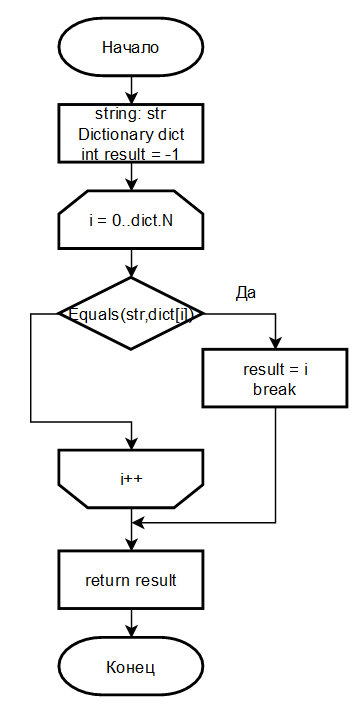
\includegraphics[scale=0.9]{source/alg1.png}
	\caption{Схема алгоритма поиска полным перебором}
	\label{Schema1}
\end{figure}
\clearpage
На \hyperref[Schema2]{рисунке 2} изображена схема алгоритма двоичного поиска.
\begin{figure}[h!]
	\centering
	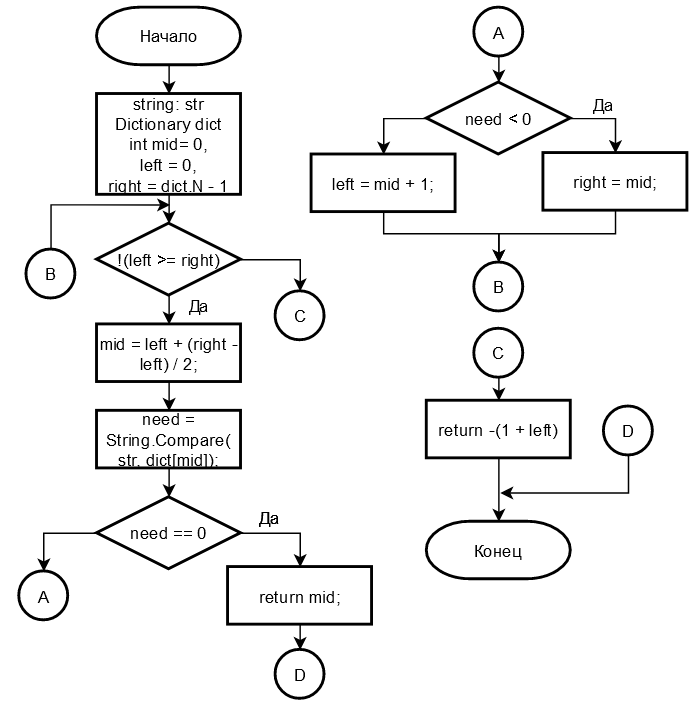
\includegraphics[scale=0.85]{source/alg2.png}
	\caption{Схема алгоритма двоичного поиска}
	\label{Schema2}
\end{figure}
\clearpage
На \hyperref[Schema3]{рисунке 3} изображена схема алгоритма поиска по сегментам.
\begin{figure}[h!]
	\centering
	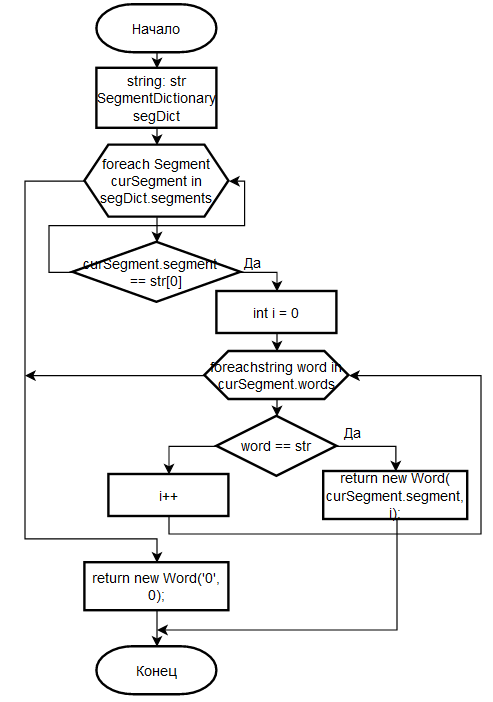
\includegraphics[scale=1]{source/alg3.png}
	\caption{Схема алгоритма поиска по сегментам}
	\label{Schema3}
\end{figure}	
\subsection{Вывод}
В данном разделе были рассмотрены схемы алгоритмов поиска.

\clearpage
\section{Технологический раздел}
В данном разделе даны общие требования к программе, средства реализации и сама реализация алгоритмов.
\subsection{Общие требования}
\textbf{Требования к вводу:}
\begin{enumerate}
	\item[1)] вводится слово;
	\item[2)] в первых 2 алгоритмах результатом будет являться ключ (в первом по обычному словарю, а во втором по отсортированному словарю), в третьем результатом будет являться ключ (первая буква или же сегмент) и индекс слова в сегменте. 
\end{enumerate}\par
\textbf{Требования к программе}
\begin{enumerate}
	\item[1)] при вводе слова, которого нет в словаре, программа не должна завершиться аварийно;
	\item[2)] ключ или же ключ-индекс должны быть корректными (соответствовать нужному слову).
\end{enumerate}
\subsection{Средства реализации}
В качестве языка программирования был выбран C\#\hyperref[literature]{[1]}, так как я знаком с данным языком программирования, имею представление о способах тестирования программы.\par
Средой разработки Visual Studio.\hyperref[literature]{[2]}\par 
Для замеров процессорного времени используется функция $Stopwatch$.\hyperref[literature]{[3]}\hyperref[literature]{[4]}\par
\subsection{Сведения о модулях программы}
Программа состоит из:
\begin{enumerate}
	\item[1)] Program.cs - главный файл программы, в котором располагается точка входа в программу;
	\item[2)] Dictionary.cs - класс, который хранит массив слов и методы для работы с этими словами;
	\item[3)] Search.cs - класс, в котором хранятся алгоритмы поиска по словарю;
	\item[4)] Segment.cs - класс сегмента, который хранит название сегмента (буква) и массив слов данного сегмента;
	\item[5)] SegmentDictionary.cs - класс, который хранит массив сегментов и методы для работы с этими сегментами;
	\item[5)] Word.cs - класс, который хранит название сегмента (буква) и индекс слова в сегменте.
\end{enumerate}
\subsection{Листинг кода программы}
В листинге 1 реализован алгоритм полного перебора слов.
\begin{lstlisting}[label=brute, caption=Алгоритм полного перебора слов]
public static int BruteForce(string str, Dictionary dict)
{
	int result = -1;
	for (int i = 0; i < dict.N; i++)
	{
		if (Equals(str, dict[i]))
		{
			return(i);
		}
	}
	return result + 1;
}	
\end{lstlisting}
В листинге 2 реализован алгоритм двоичного поиска.
\begin{lstlisting}[label=binary, caption=Алгоритм двоичного поиска]
public static int BinaryFind(string str, Dictionary dict)
{
	int result, left = 0, right = dict.N - 1;
	while (true)
	{
		if (left > right)
		{
			return 0;
		}
		result = left + (right - left) / 2;
		int need = String.Compare(str, dict[result]);
		if (need < 0)
		{
			right = result + 1;
		}
		if (need > 0)
		{
			left = result - 1;
		}
		if (need == 0)
		{
			return result;
		}
	}
}
\end{lstlisting}
В листинге 3 реализован алгоритм поиска по сегментам.
\begin{lstlisting}[label=segment, caption=Алгоритм поиска по сегментам]
public static Word FindInSegment(string str, SegmentDictionary segDict)
{
	foreach (Segment curSegment in segDict.segments)
	{
		if (curSegment.segment == str[0])
		{
			int i = 0;
			foreach (string word in curSegment.words)
			{
				if (word == str)
				{
					return new Word(curSegment.segment, i);
				}
				i++;
			}
			return new Word('0', 0);
		}
	}
	return new Word('0', 0);
}
\end{lstlisting}
\subsection{Вывод}
В данном разделе были даны общие требования к программе, описаны средства реализации, были представлены сведения о модулях программы, а также реализованы алгоритмы поиска по словарю.

\clearpage
\section{Экспериментальный раздел}
В данном разделе представлены результаты работы программы и приведен анализ времени работы алгоритмов.
\subsection{Описание экспериментов}
Производится замер времени для $n + 1$ возможных случаев, где $n$ - длина словаря. 
\subsection{Примеры работы программы}
На \hyperref[Example1]{рисунке 4} представлен результат работы алгоритмов.
\begin{figure}[h!]
	\centering
	\includegraphics[scale=1]{source/Example.png}
	\caption{Первый результат работы программы}
	\label{Example1}
\end{figure}\par
На \hyperref[Test1]{рисунке 5} представлены результаты сравнения трех алгоритмов поиска.
\begin{figure}[h!]
	\centering
	\begin{tikzpicture}[object/.style={thin,double,<->}]
		
		\begin{axis}[
			axis lines = left,
			xlabel = $\textit{индекс слова в словаре}$,
			ylabel = {$\textit{время (тики)}$},
			legend pos=north west,
			ymajorgrids=true
			]
			\addplot[color=red] table[x index=0, y index=1] {source/BruteForce.dat}; 
			\addplot[color=orange] table[x index=0, y index=1] {source/BinaryFind.dat};
			\addplot[color=blue, mark=square] table[x index=0, y index=1] {source/FindInSegment.dat};
			
			\addlegendentry{Полный перебор}
			\addlegendentry{Бинарный поиск}
			\addlegendentry{Поиск по сегментам}
			
		\end{axis}
	\end{tikzpicture}
	
	\caption{Результаты замеров процессорного времени.}
	\label{Test1}
\end{figure}\par
\newpage
\subsection{Вывод}
Результаты тестирования показывают, что самым эффективным и "стабильным" является бинарный поиск. Самым долгим является алгоритм полного перебора. Его время возрастает каждый раз из-за того, что слова находятся дальше в словаре, а каждый поиск начинается с самого начала. По графику алгоритма поиска по сегментам можно увидеть резкие скачки. Это происходит из-за того, что слово в находится в конце сегмента. Можно сделать вывод, что самым эффективным является алгоритм бинарного поиска.
\clearpage
\section{Заключение}
В ходе выполнения данной лабораторной работы были изучены три алгоритмы поиска по словарю. Были описаны все алгоритмы и реализованы. Также были изучены способы хранения слов, то есть в случаях первого и второго алгоритмов слова хранились в массивах, а в третьем хранилось по сегментам. Сравнили время работы алгоритмов, в результате которого стало понятно, что самым эффективным алгоритм был бинарный поиск.
\clearpage
\section*{Литература}
\addcontentsline{toc}{section}{Литература}
\begin{enumerate}
	\label{literature}
	\item  Документация по C\#. -URL: \href{https://docs.microsoft.com/ru-ru/dotnet/csharp/}{https://docs.microsoft.com/ru-ru/dotnet/csharp/} (дата обращения: 24.10.2020). -Текст: электронный.
	\item Документация по семейству продуктов Visual Studio. -URL:\par \href{https://docs.microsoft.com/ru-ru/visualstudio/?view=vs-2019}{https://docs.microsoft.com/ru-ru/visualstudio/?view=vs-2019 } (дата обращения: 01.10.2020). -Текст: электронный.
	\item Stopwatch Класс. -URL: \href{https://goo.su/2e99}{https://goo.su/2e99 } (дата обращения: 24.10.2020). -Текст: электронный.
	\item Под капотом у Stopwatch. -URL:  \href{https://habr.com/ru/post/226279/}{https://habr.com/ru/post/226279/} (дата обращения: 24.10.2020). Текст: электронный.
\end{enumerate}
\end{document}\par